\section{Canonical Form and the \texorpdfstring{$\kappa \leftrightarrow 1/\kappa$}{kappa <-> 1/kappa} Symmetry}
\label{sec:canonical}

\subsection{The Change of Variables}

Fisher's paired efficiency \parencite{fisher1935} is the benchmark case $\kappa = 1$; when the two margins differ, the ratio-of-variances literature \parencite{bose1935} and the Pitman--Morgan test for equal paired variances \parencite{pitman1939,morgan1939} address related distributional questions but not the canonical efficiency coordinate developed below.

The Paired Efficiency Factor \parencite{brownPEFempirical} is defined as the ratio of unpaired to paired variance,
\begin{equation}
  \eta(\kappa,\rho)
  = \frac{1+\kappa}{1+\kappa-2\sqrt{\kappa}\,\rho},
  \label{eq:pef_original}
\end{equation}
where $\kappa = \sigma_{\mathrm{B}}^{2}/\sigma_{\mathrm{A}}^{2} > 0$ is the variance ratio and $\rho \in (-1,1)$ is the Pearson correlation between the two margins.
In the sports datasets of \textcite{brownPEFempirical}, each index is one fixture.
Then $\hat\rho$ is the cross-fixture correlation of the home and away values, not serial correlation of one team's series.
Set
\begin{equation}
  \tau = \tfrac{1}{2}\log\kappa,
  \label{eq:tau_def}
\end{equation}
so that $\sqrt{\kappa} = e^{\tau}$.
Dividing the numerator and the denominator of \cref{eq:pef_original} by $\sqrt{\kappa}$ gives the canonical form.
The algebra is in \cref{sec:appendix_canonical}.
\begin{equation}
  \eta(\tau,\rho)
  = \frac{\cosh\tau}{\cosh\tau - \rho}.
  \label{eq:canonical}
\end{equation}
Here $\tau \in \mathbb{R}$ measures variance asymmetry on a symmetric log-scale, and $\rho$ remains the correlation.
The half-strip $\{\tau \ge 0,\, \rho \in (-1,1)\}$ is the fundamental domain: $\kappa \ge 1$ maps onto it bijectively.
The identity $\eta = 1/(1-u)$ with $u = \rho\,\sech\tau$ is \cref{eq:u_def}.
The remarks in \cref{sec:scalar} and the sampling theory in \cref{sec:sampling} use only this identity.

\Cref{fig:halfstrip_domain} shows the fundamental half-strip with iso-$\eta$ contours and the involution that folds the four empirical quadrants onto $\tau\ge 0$.

\begin{figure}[t]
  \centering
  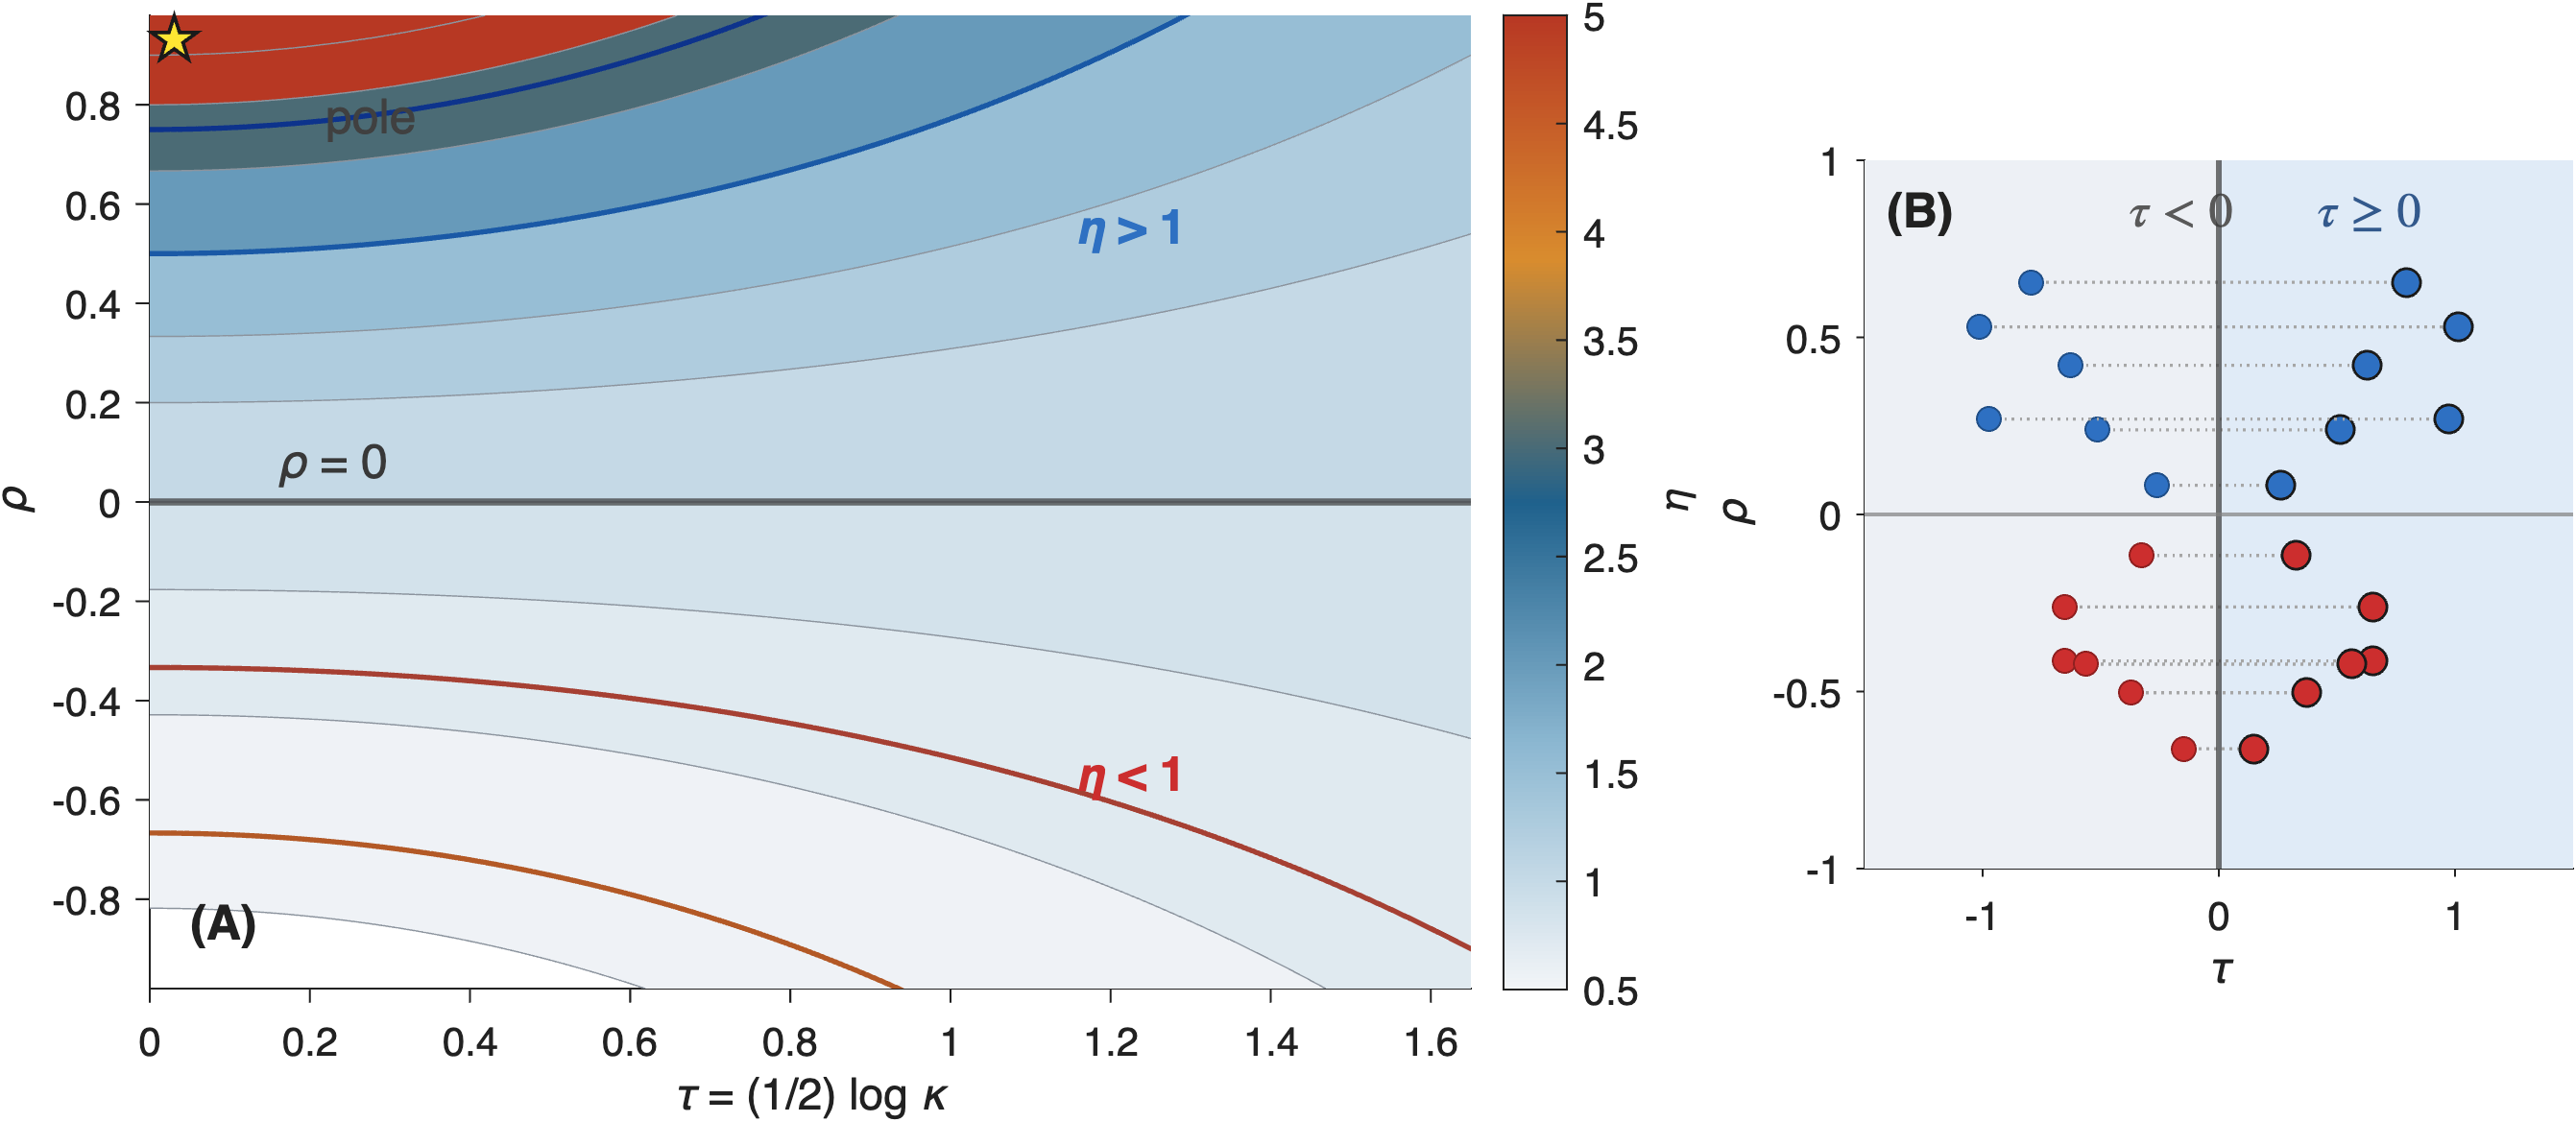
\includegraphics[width=\textwidth]{figures/Figure_1_halfstrip_domain.png}
  \caption{Canonical form on the half-strip $\tau\ge 0$.
    (A)~Iso-$\eta$ contours.
    The left boundary is the Fisher line $\tau=0$.
    The horizontal line is $\rho=0$, where $\eta=1$.
    The star marks the pole approached as $(\tau,\rho)\to(0,1)$.
    (B)~The involution $\tau\mapsto-\tau$ identifies $\kappa$ with $1/\kappa$ at fixed $\rho$, so $\eta$ is unchanged.}
  \label{fig:halfstrip_domain}
\end{figure}

\subsection{The \texorpdfstring{$\kappa \leftrightarrow 1/\kappa$}{kappa <-> 1/kappa} Involution}

\begin{theorem}[Involution]
\label{thm:involution}
For all $\kappa > 0$ and $\rho \in (-1,1)$ with $\cosh\tau \ne \rho$,
\[
  \eta(\kappa,\rho) = \eta(1/\kappa,\rho).
\]
\end{theorem}

\begin{proof}
Substituting $\kappa \mapsto 1/\kappa$ replaces $\tau = \tfrac{1}{2}\log\kappa$ by $-\tau$.  Since $\cosh$ is even, $\cosh(-\tau)=\cosh\tau$, and the right-hand side of \cref{eq:canonical} is unchanged.
\end{proof}

\begin{corollary}
The map $\kappa \mapsto 1/\kappa$ is an involution of the parameter space, and it fixes $\eta$.
The empirical cells of \textcite{brownPEFempirical} split on the signs of $\kappa-1$ and of $\rho$.
The involution exchanges the two cells with $\rho>0$, and the two cells with $\rho<0$.
It does not exchange the sign of $\rho$.
\end{corollary}

On the paired estimates from that paper, $|\hat\eta(\kappa,\rho)-\hat\eta(1/\kappa,\rho)|$ is at most $1.78\times 10^{-15}$ (\cref{sec:numerical}).
That residual checks the implementation of \cref{thm:involution}.
It is not an empirical test of the identity.

\subsection{Domain and Singularity Locus}

The denominator $\cosh\tau - \rho$ vanishes when $\rho = \cosh\tau \ge 1$, which is outside the physical domain $\rho \in (-1,1)$ except at the single boundary point $(\tau,\rho) = (0,1)$, where $\eta \to +\infty$.  Near this pole, set $\tau = \varepsilon_1$ and $\rho = 1 - \varepsilon_2$ with $\varepsilon_1, \varepsilon_2 \to 0^+$.  Then $\cosh\tau - \rho \approx (1 + \tfrac{1}{2}\varepsilon_1^2) - (1-\varepsilon_2) = \varepsilon_2 + \tfrac{1}{2}\varepsilon_1^2$, giving the local parabolic blow-up
\begin{equation}
  \eta \;\approx\; \frac{1}{(1-\rho) + \tfrac{1}{2}\tau^{2}}.
  \label{eq:parabolic_blowup}
\end{equation}
Iso-$\eta$ contours near the pole are therefore parabolas $1-\rho = C - \tfrac{1}{2}\tau^{2}$ in the $(\tau,\rho)$-plane.
The same blow-up is the local form of $\eta = 1/(1-u)$ as $u\to 1$.

\subsection{Differential Structure}

From \cref{eq:canonical},
\begin{align}
  \frac{\partial\eta}{\partial\rho}
  &= \frac{\cosh\tau}{(\cosh\tau-\rho)^{2}} > 0,
  \label{eq:deta_drho}\\[4pt]
  \frac{\partial\eta}{\partial\tau}
  &= \frac{\sinh\tau\,(\cosh\tau-\rho) - \cosh\tau\,\sinh\tau}{(\cosh\tau-\rho)^{2}}
   = -\,\frac{\rho\,\sinh\tau}{(\cosh\tau-\rho)^{2}}.
  \label{eq:deta_dtau}
\end{align}
Thus $\eta$ is strictly increasing in $\rho$ for every $\tau$.
The sign of $\partial\eta/\partial\tau$ is opposite to the sign of $\rho\,\tau$.
For $\rho>0$, $\eta$ decreases towards $1$ as $|\tau|$ grows.
For $\rho<0$, $\eta$ increases towards $1$ as $|\tau|$ grows.
Variance asymmetry therefore pulls $\eta$ towards the correlation-free value $1$ in both cases.
This matches the limit $\eta\to 1$ as $|\tau|\to\infty$ in \cref{tab:special_values}.
The critical set $\partial\eta/\partial\tau = 0$ is the union of the lines $\tau = 0$ and $\rho = 0$.
Sensitivity to correlation, measured by \cref{eq:deta_drho}, is largest at $\tau = 0$ and decays as $|\tau|\to\infty$.

\subsection{Special Values}
\label{sec:special_values}

\begin{table}[t]
  \centering
  \caption{Boundary behaviour of the canonical form~\cref{eq:canonical}.}
  \label{tab:special_values}
  \begin{tabular}{@{}llll@{}}
    \toprule
    \textbf{Condition} & \textbf{$\tau$} & $\eta$ & \textbf{Note} \\
    \midrule
    $\kappa = 1$ (Fisher case) & $0$ & $\dfrac{1}{1-\rho}$ & Classical formula \\[6pt]
    $\rho = 0$                 & any & $1$                   & Correlation-free baseline \\[2pt]
    $\rho \to +1$              & $0$ & $+\infty$             & Perfect pairing, equal variances \\[2pt]
    $\rho \to -1$              & $0$ & $\tfrac{1}{2}$        & Maximum variance amplification \\[2pt]
    $\kappa \to 0$ or $\infty$ & $|\tau| \to \infty$ & $1$ & Extreme asymmetry collapses to baseline \\
    \bottomrule
  \end{tabular}
\end{table}

A notable identity follows from evaluating \cref{eq:canonical} at $\rho = +1$ and $\rho = -1$:
\begin{equation}
  \eta(\tau,+1)\cdot\eta(\tau,-1)
  = \frac{\cosh\tau}{\cosh\tau-1}\cdot\frac{\cosh\tau}{\cosh\tau+1}
  = \frac{\cosh^{2}\tau}{\cosh^{2}\tau-1}
  = \frac{\cosh^{2}\tau}{\sinh^{2}\tau}
  = \coth^{2}\tau.
  \label{eq:reciprocal_product}
\end{equation}
At $\tau = 0$ (Fisher's case), $\coth\tau \to \infty$, reflecting the pole.  For large $|\tau|$, $\coth\tau \to 1$, so the product approaches unity: the efficiency gain at maximal positive correlation is asymptotically the reciprocal of the efficiency loss at maximal negative correlation.  This is a residual echo of the involution.

\subsection{Consequence for the Empirical Four-Quadrant Taxonomy}
\label{sec:quadrant_coverage}

The empirical paper partitions the $(\kappa,\rho)$-plane by the signs of $\kappa-1$ and $\rho$.
\Cref{thm:involution} shows that $\eta$ does not distinguish $\kappa$ from $1/\kappa$.
The cells that differ only by which margin is more variable therefore share a value of $\eta$.
They do not share a predictive comparison.
The empirical comparator is the labelled series $X_{\mathrm{A}}$.
Under the swap $\mathrm{A}\leftrightarrow\mathrm{B}$, the relative signal $d_{\mathrm{rel}}$ and the correlation $r_{\mathrm{A}} = \Corr(X_{\mathrm{A}},X_{\mathrm{A}}-X_{\mathrm{B}})$ change.
On the sports estimates those two coordinates differ by a factor $\sqrt{\kappa}$ that runs from $0.761$ to $1.160$, so one labelling can sit $24\%$ away from the other (\cref{sec:numerical}).
The cell split on $\kappa=1$ is empty for efficiency.
It is not empty for a comparison that uses $X_{\mathrm{A}}$.
